\chapter{ MARCO TEORICO }
\section{Métodos para estimar la capacidad eléctrica de las baterías}

Tradicionalmente, los ciclos de carga y descarga han constituido un método clásico de medición de la capacidad eléctrica de las baterías. Adicionalmente, se han intentado utilizar métodos alternativos, pero sin resultados fidedignos para los usuarios. Estas incertidumbres han llevado a los usuarios a quedarse con los métodos de descarga tradicionales, a pesar de su desventaja principal, la cual es remover la batería del sistema para poder estimar su capacidad eléctrica~\cite{Buchmann2011}. A continuación, se mencionarán dos métodos para estimar la capacidad eléctrica de las baterías. Cabe resaltar que existen diversos métodos para analizar las baterías, sin embargo, solo se van a mencionar aquellos que involucren la estimación de la capacidad eléctrica de las baterías y no en la estimación del tiempo de vida, estado de carga, estado de salud, ni otros parámetros que caracterizan a las baterías. \\

\textbf{\underline{Método de descarga}}

Se suele pensar que el método de descarga es el método más preciso para estimar la capacidad eléctrica de las baterías, sin embargo, esto no siempre ocurre, especialmente con las baterías de plomo ácido. Este método sufre variaciones en los resultados, incluso con pruebas idénticas de equipos de alta precisión que fueron utilizados en ambientes de temperatura controlados y siguiendo los estándares de descarga establecidos. Así mismo, esto se refleja en dos pruebas idénticas que se realizó a varias baterías de arranque cuyos resultados se pueden observar en la figura ~\ref{fig:testidentica}. El eje horizontal indica, de izquierda a derecha, las baterías más débiles hasta las más potentes y el eje vertical muestra la capacidad eléctrica que las baterías presentaron. Las dos pruebas se realizaron bajo las mismas condiciones, pero la segunda se realizó pocos días después de haber finalizado la primera. Los resultados muestran que la capacidad eléctrica del mismo tipo de batería tuvo variaciones en algunos puntos~\cite{measurecapacity}.

\begin{figure}[htbp]
\begin{center}
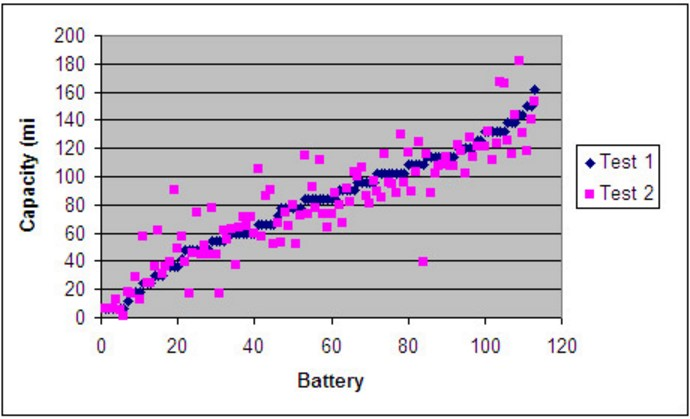
\includegraphics[width=12cm]{CAP2_testidentica.jpg}
\caption{Fluctuaciones de la capacidad eléctrica como resultado de dos idénticas pruebas de acuerdo a los estándares SAE J535~\cite{Buchmann2011}.}
\label{fig:testidentica}
\end{center}
\end{figure}

Sin embargo, la mayoría de estos resultados y comentarios son aplicados para las baterías en general, pero dentro de esta incertidumbre los que muestran resultados más consistentes son las baterías tipo li-ion. Esto se debe a que los ciclos de carga y descarga afectan a la capacidad eléctrica, en mayor medida, a los tipos de batería ácido plomo; mientras que, las baterías Li-ion pueden tener entre 300 y 500 ciclos de carga y descarga sin afectar mucho a su capacidad eléctrica~\cite{capacityloss}. Así mismo, teniendo en cuenta la ilustración 1, el desempeño de la batería Ni-MH, el cual presenta similitudes en el comportamiento de las baterías Li-ion, se observa que, para descargas analógicas y descargas estandarizadas por el IEC, la capacidad eléctrica de la batería no varía mucho en los primeros ciclos de carga y descarga~\cite{Buchmann2011}. \\

El funcionamiento del método de descarga se basa en aplicar una descarga a la batería con la finalidad de medir su tiempo de operación. Los instrumentos actuales en el mercado manejan cuatro tipos de descarga:

\begin{enumerate}
\item Descarga a Corriente Constante
\item Descarga a Voltaje Constante
\item Descarga a Potencia Constante
\item Descarga a Resistencia Constante
\end{enumerate}

Los cuatros métodos coinciden en mantener una variable constante de tal manera que la descarga de la batería tenga un parámetro constante durante todo su tiempo de operación. Luego de conocer el tiempo que duró la batería, se utiliza el parámetro constante para hallar la capacidad eléctrica de la batería en mAh. \\

\textbf{\underline{Método no Invasivo}}

El método no Invasivo utiliza múltiples modelos de espectroscopia de impedancia electroquímica (EIS, por sus siglas en inglés) con la finalidad de estimar el estado de la carga (SoC), la capacidad eléctrica y la corriente de arranque en frio, más conocido como Cold Cranking Amp (CCA). El CCA indica la capacidad de poder conducir altas corrientes en las baterías de arranque. El funcionamiento de este método se basa en introducir varias señales sinusoidales con poca amplitud a diferentes frecuencias, para luego utilizar un filtrado digital y de las señales extraídas se forma una curva de Nyquist. Luego, encima de la curva de Nyquist formada, se superpone varios modelos electro químicos con la finalidad de correlacionar la información y obtener los parámetros clave que indicarán la estimación de la capacidad eléctrica, CCA y SoC~\cite{measurecapacity}. 

\begin{figure}[htbp]
\begin{center}
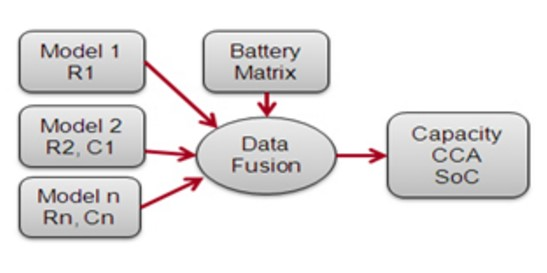
\includegraphics[width=12cm]{CAP2_metodonoinvasivo.jpg}
\caption{Método no Invasivo que implica la combinación de EIS con modelos complejos para estimar la capacidad de la batería~\cite{measurecapacity}}
\label{fig:metodonoinvasivo}
\end{center}
\end{figure}

Luego de comprender ambos métodos para la estimación de la capacidad eléctrica de las baterías, se evalúan las ventajas y desventajas de éstas. En el cuadro~\ref{tab:comparacionmetodos}, se puede apreciar que utilizar el método no invasivo implica realizar subprocesos complejos que incrementarían los costos del instrumento a diseñar. Por ello, para la presente tesis, se procede a utilizar el método de descarga cuyos resultados son consistentes en el tipo de batería Li-ion.

%cuadro comparación metodos
\begin{table}[htbp]
\caption{Comparación de ventajas y desventajas entre el método de descarga y el método no invasivo~\cite{measurecapacity}}
\begin{center}
\begin{tabular}{|c|L{6cm}|L{5cm}|}\cline{2-3}
\multicolumn{1}{c|}{}&\multicolumn{1}{c|}{Ventajas}&\multicolumn{1}{|c|}{Desventajas}\\\hline
\multicolumn{1}{|c|}{\multirow{2}{*}{Método de Descarga}}&\tabitem Es un método práctico para hallar la capacidad eléctrica de la batería&\tabitem Se debe trasladar la batería al instrumento para realizar el análisis\\
&\tabitem Los resultados son consistentes en baterías Li-ion& \tabitem El proceso toma un tiempo considerable\\\hline
\multicolumn{1}{|c|}{\multirow{2}{*}{Método no Invasivo}}&\tabitem El proceso de análisis se puede realizar en segundos &\tabitem Es un método que permite estimar otros parámetros de la batería\\
&\tabitem Es un método muy complejo de implementar& \tabitem Requiere mayores costos para realizarlo\\\hline
\end{tabular}
\end{center}
\label{tab:comparacionmetodos}
\end{table}


\section{Instrumentos actuales de medición para baterías}

En la actualidad, diferentes empresas de todo el mundo utilizan instrumentos de medición para medir la capacidad eléctrica de las baterías. Por ejemplo, entre las empresas más destacadas se encuentran Cadex, Mayuno Electronic, Tektronix y National Instruments. Si bien los instrumentos de medición de estas empresas difieren en características técnicas, todos ellos comparten en común el método de descarga como una alternativa para determinar la capacidad eléctrica de las baterías.\\

Dado que el objetivo de la tesis implica el diseño de un instrumento de medición para baterías, se resalta las características principales de éstos que servirán como referencia para el diseño propio. Entre las características principales se encuentra:

\begin{itemize}
\item\underline{Rango de operación de la batería:} El rango de voltajes de la batería en el que opera el instrumento
\item\underline{Rango de de descarga de corriente:} La máxima y mínima corriente que el instrumento puede descargar
\item\underline{Resolución de medida:} La resolución de un isntrumento es el menor incremento de la variable medida, la cual es determinado por el ADC y DAC
\item\underline{Exactitud:} La exactitud es aquella característica que define el rango de valores de incertidumbre al momento de hacer una lectura
\end{itemize}

Luego de haber revisado los detalles más importantes que tienen los instrumentos de medición, se realizó el cuadro~\ref{tab:instrumentos} con la finalidad de poder comparar los valores de las características antes mencionadas. Así mismo, se incluye los periféricos de entrada y salida que muestran la información de la capacidad eléctrica una vez realizado todo el proceso (display y data ports).

%cuadro comparacion instrumentos comerciales

\begin{table}[htbp]	
\begin{adjustwidth*}{-1cm}{-1cm}
    \centering
\renewcommand{\arraystretch}{1}
\setlength\tabcolsep{3pt}
\scriptsize
    \caption{Comparación de características entre los instrumentos actuales para baterías en el mercado}
\begin{tabularx}{\linewidth}{| L{2cm} |
            >{\hsize=0.9\hsize}C |       
                        *{3}{C |}
            >{\hsize=1.1\hsize}C |
                             }
    \cline{2-6}
\multicolumn{1}{c|}{}
    &   \textbf{Cadex C7600~\cite{Cadexcompany}} 
        &   \textbf{Cadex C8000~\cite{Company}} 
            &   \textbf{NI PXI-4130~\cite{NationalInstruments2000}} 
                &   \textbf{Tektronix 2380~\cite{KEITHLEYaTektronixCompany}} 
                    &   \textbf{Maynuo M9712C~\cite{MaynuoElectronic}}              \\
    \hline
Battery voltage range   
    & \SIrange{1.2}{36}{V} & \SIrange{1.2}{36}{V} & \SIrange{0}{20}{V} 
        & \SIrange{0}{500}{V} & \SIrange{0.1}{150}{V} \\
    \hline
\multirow{4}{=}{Discharge method}
    &   \multirow{4}{*}{Constant current} 
        &   \multirow{2}{*}{Constant current} 
            &   \multirow{2}{*}{Constant current} 
                &   Constant current 
                    &   Constant current            \\  
    &   &   &   &   Constant voltage 
                    &   Constant voltage            \\ 
    &   &   \multirow{2}{*}{Constant power} 
            &   \multirow{2}{*}{Constant voltage} 
                    &   Constant resistance 
                        &   Constant resistance     \\ 
    &   &   &   &   Constant power 
                        & Constant power            \\
    \hline
Range of discharge current
    & \SIrange{0.1}{6}{A} & \SIrange{0.03}{10}{A} 
        & \SIrange{2}{20}{mA} & \SIrange{0}{15}{A} & \SIrange{0}{6}{A}  \\
    \hline
Resolution       
    & \SI{25}{mA} & \SI{1}{mA} & \SI{100}{nA} & \SI{1}{mA} & \SI{0.01}{mA} \\
    \hline
Exactitud        
    & \SI{0.25}{\%} FS & \SI{0.25}{\%} FS & \SI{0.03}{\%} FS 
        & (\SI{0.05}{\%} FR + \SI{0.05}{\%} FS) & \SI{0.015}{\%} FR + \SI{0.05}{\%} FS \\
    \hline
Operating Temperature
    & \SIrange{5}{35}{\degreeCelsius} & \SIrange{5}{35}{\degreeCelsius} 
        & \SIrange{0}{55}{\degreeCelsius} & \SIrange{0}{40}{\degreeCelsius} 
            & \SIrange{0}{40}{\degreeCelsius}\\
    \hline
Display  & 2x40-character LCD & \SI{5.7}{''} (145mm) QVGA 320x240 graphics with backlight & There isn’t available information & Monitor Output BNC & High-luminance VFD screen with two line \\
    \hline
Data ports  & RS-232 or USB interfaces to PC & Ethernet 10/100 MB for connection to PC & There isn’t available information & USB, RS-232, GPIB & USB, RS232, RS485 \\
    \hline
\end{tabularx}
\label{tab:instrumentos}
\end{adjustwidth*}
\end{table}

FS: Full Scale \\	
FR: For Reading \\	
VFD: Vacuum Fluorescent display \\

En cuanto a la resolución y exactitud de los instrumentos del cuadro~\ref{tab:instrumentos}, se puede apreciar que a medida que haya mayor rango de descarga de corriente, la resolución va disminuyendo. Por ejemplo, en el instrumento de National Instruments PXI-4130 se observa que tiene una resolución increíble de 100 nA, sin embargo, su rango de descarga es mucho menor que los demás instrumentos de medición. Otro ejemplo es la comparación entre los instrumentos Tektronix 2380 y Maynuo M9712C; ya que, el instrumento de Tektronix brinda un mayor rango de descarga de corriente, pero con menor resolución. Este tipo de comparación no aplica entre los instrumentos Cadex C7600 y C8000 debido a que éste último es una versión mejorada del instrumento en general. Además, en cuanto a la exactitud, se puede observar que los instrumentos manejan sistemas de adquisición avanzados para conseguir un pequeño error en las medidas realizadas. Éste último podría justificar sus elevados costos en el mercado, además de que varios de estos instrumentos ofrecen otras funciones aparte del método de descarga.

\section{Estructura de los instrumentos de medición para baterías}

Una vez identificado las características principales de los instrumentos de medición para baterías, se busca comprender las diferentes estructuras de estos instrumentos con la finalidad de tenerlos como referencia para el diseño del prototipo que propone la tesis. Para ello se revisaron las patentes del instrumento de la compañía Cadex y algunos diagramas de bloques generales que se basaron en sistemas de estimación de la capacidad eléctrica de las baterías. \\

En la figura~\ref{fig:patenteref} se muestra un diagrama de bloques de la patente de un instrumento de medición de la compañía Cadex. El sistema representado por este diagrama de bloques funciona a través de ciclos de carga y descarga de la batería, cuyos datos son adquiridos, procesados y guardados por un controlador. En adición, presenta un periférico de salida en el bloque 212 y los datos son almacenados en una base de datos representado por el bloque 203. En la patente no se desarrollan los bloques debido a que le dan mayor énfasis al método de lógica difusa para estimar el estado de la batería. Sin embargo, se resalta que este sistema tiene una etapa de adquisición, proceso y almacenamiento~\cite{Tinnemeyer}. \\

\begin{figure}[!ht]
\begin{center}
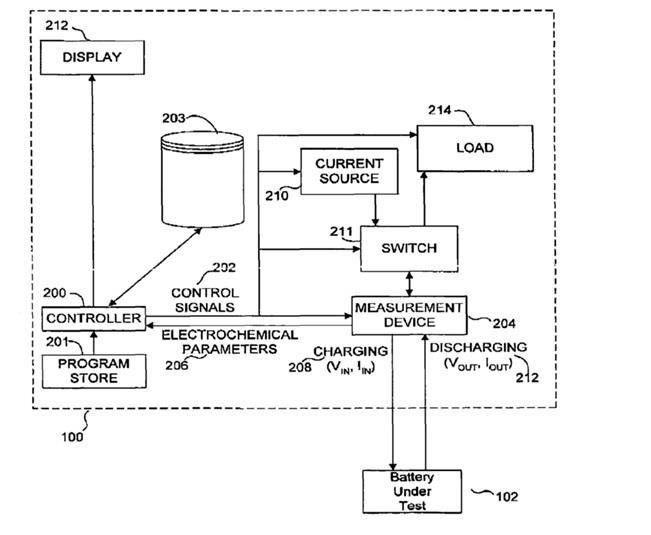
\includegraphics[width=12cm]{CAP2_patenteref.jpg}
\caption{Diagrama de bloques de una patente del instrumento de medición para baterías de la compañía Cadex~\cite{Tinnemeyer}.}
\label{fig:patenteref}
\end{center}
\end{figure}

Por otro lado, se analiza dos publicaciones de la IEEE basados en sistemas de estimación de los parámetros de las baterías. \\

En la primera publicación, el sistema busca una estimación del estado de salud y el tiempo de vida de las baterías. El diagrama de bloques de esta publicación, como se muestra en la figura~\ref{fig:diagbloquesref}, consiste en descargar la batería y tomar los datos que serán procesados por una computadora. Se identifica tres etapas en el diagrama de bloques, las cuales son: etapa de control, etapa de adquisición y monitoreo de temperatura. La etapa de control representada por el bloque 1 sirve para mantener controlado la descarga de la batería; así mismo, la etapa de adquisición representado por el bloque 2 consiste en adquirir los valores de corriente durante todo el tiempo de operación de la batería; por último, la etapa de monitoreo representada por el bloque 3 consiste en medir la temperatura durante todo el proceso con la finalidad de tenerlo de referencia en los resultados~\cite{Harris2015}. \\

\begin{figure}[!ht]
\begin{center}
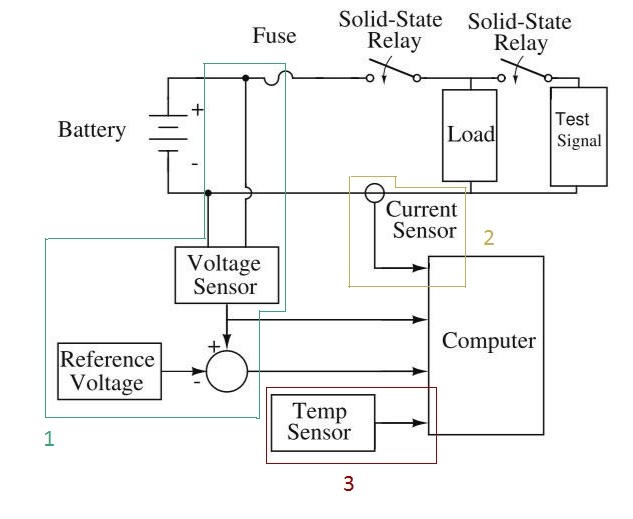
\includegraphics[width=12cm]{CAP2_diagbloquesref.jpg}
\caption{Diagrama de bloques de un instrumento de medición que estima el estado de salud y el tiempo de vida de la batería~\cite{Harris2015}.}
\label{fig:diagbloquesref}
\end{center}
\end{figure}

La segunda publicación consiste en la estimación de la impedancia interna mediante el método de doble descarga en baterías ácido plomo. En la figura~\ref{fig:diagramaref} se puede apreciar el diagrama de bloques que está constituido por un controlador C8051F, una PC, el método de descarga a corriente constante y un seleccionador de celdas. La PC representaría la etapa de proceso de datos; mientras que, el controlador C8051F representaría la etapa de adquisición y de control de celdas de la batería; por último, la etapa de descarga mediante el método de descarga de corriente constante por el cual se obtendrán los datos para estimar la capacidad eléctrica de la batería~\cite{Ping2012}. 

\begin{figure}[!ht]
\begin{center}
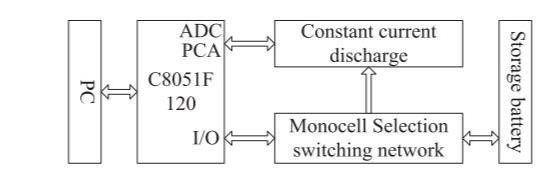
\includegraphics[width=12cm]{CAP2_diagramaref.jpg}
\caption{Diagrama de bloques de un sistema de medición on-line para baterías plomo ácido~\cite{Ping2012}.}
\label{fig:diagramaref}
\end{center}
\end{figure}

Luego de haber analizado las estructuras de los instrumentos de medición para baterías, se puede observar que comparten ciertos patrones en los diagramas de bloques. El primero es que se considera una etapa de almacenamiento y procesamiento de datos para cualquier instrumento; así mismo, se identifica un segundo patrón que consiste en la etapa de adquisición de datos, ya sea voltaje o corriente que permitan la estimación de la capacidad eléctrica de la batería; por último, se identifica un tercer patrón sobre un sistema de control para los métodos de descarga, ya que el voltaje de las baterías varía mientras se descarga. Además, se puede mencionar que hay dos tipos de bloques: los bloques que influyen de manera directa a la estimación de la capacidad eléctrica de la batería y otros bloques complementarios que están para el adecuado funcionamiento del instrumento. Un ejemplo del primer tipo de bloque sería la etapa de adquisición ya que en este bloque se evalúa la incertidumbre de las medidas tomadas para la capacidad eléctrica. Mientras que, un ejemplo del segundo tipo de bloque sería la etapa de monitoreo de temperatura debido a que las medidas de temperaturas adquiridas no afectan a la estimación de la capacidad eléctrica de la batería. \\

De este modo, el diagrama propuesto que se desarrollará en el diseño del instrumento debe constituir tener incluido los siguientes bloques:

\begin{itemize}
\item Etapa de procesamiento y almacenamiento
\item Etapa de adquisición de datos
\item Etapa de monitoreo de temperatura
\item Etapa de control del método de descarga
\end{itemize}

El diseño de cada bloque será desarrollado en el capítulo tres a través de los conocimientos adquiridos en los cursos de Circuitos Analógicos, Diseño Electrónico y Circuitos Eléctricos. No obstante, el bloque de control del método de descarga requiere una mayor profundización teórica debido a que es bloque fundamental por el cual se obtendrán los datos para estimar la capacidad eléctrica de las baterías Li-ion y pilas alcalinas. 

\section{Topologías del sistema de control del método de descarga}

En la sección 2.1 se evaluaron las ventajas y desventajas de los métodos de estimación de la capacidad eléctrica, por los cuales se establece que el método a utilizar en la presente tesis es el método tradicional de descarga debido a que es práctico y presenta resultados consistentes para baterías Li-ion en sus primeros ciclos de carga y descarga. Así mismo, se definió que había cuatro tipos de descarga: voltaje constante, corriente constante, resistencia constante y potencia constante. Debido a que, por lo general, la medida del consumo de los sistemas realizados en los proyectos académicos o de investigación se utiliza la corriente, el método de descarga a utilizar será el de corriente constante. \\

El método de descarga a corriente constante consiste en conectar una carga a la batería de tal manera que consuma una corriente constante a pesar de las variaciones del voltaje que haya en la batería, ya que como se revisó en el capítulo 1, el voltaje de referencia de la batería va disminuyendo a medida que se descarga. Para ello, se verán diferentes topologías de circuitos que permitan el control de la corriente constante. \\

\begin{figure}[!ht]
\begin{center}
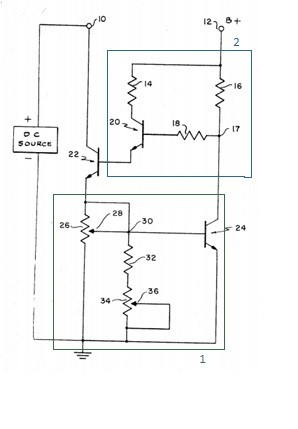
\includegraphics[width=12cm]{CAP2_patenteford.jpg}
\caption{Circuito de descarga de corriente constante publicado en la patente de F.E. Ford~\cite{FordFloydE.1966}.}
\label{fig:patenteford}
\end{center}
\end{figure}

Una patente publicada en 1969 por Ford Floyd describe el funcionamiento del control para obtener una descarga de corriente constante. Pues como se aprecia en la figura~\ref{patenteford}, el terminal positivo de la batería se conecta en el nodo 10 y el terminal negativo a tierra, luego por medio de los bloques 1 y 2 se realiza el control. El bloque 1 sería la realimentación del circuito y el bloque 2 funcionaría como el circuito que activa el transistor 22, el cual permite el paso de la corriente por la carga. La corriente descargada estaría sujeto al voltaje del colector del transistor 24~\cite{FordFloydE.1966}. Lo fundamental de esta topología es reconocer que se utiliza un transistor NPN para generar la corriente constante; además, existe una realimentación en el sistema para conseguir el control y una etapa de activación para el transistor NPN.\\

Se presentan 3 topologías adicionales que han formado parte de publicaciones recientes. \\

\begin{figure}[!ht]
\begin{center}
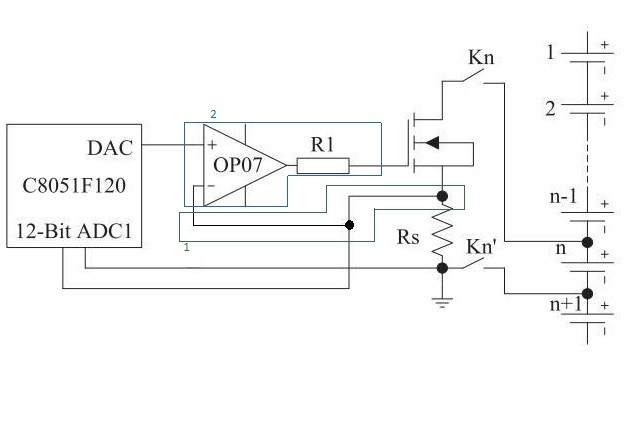
\includegraphics[width=12cm]{CAP2_cktoreferencia.jpg}
\caption{Circuito modificado de descarga de corriente constante para una celda de batería~\cite{Ping2012}.}
\label{fig:cktoreferencia}
\end{center}
\end{figure}

\begin{figure}[!ht]
\begin{center}
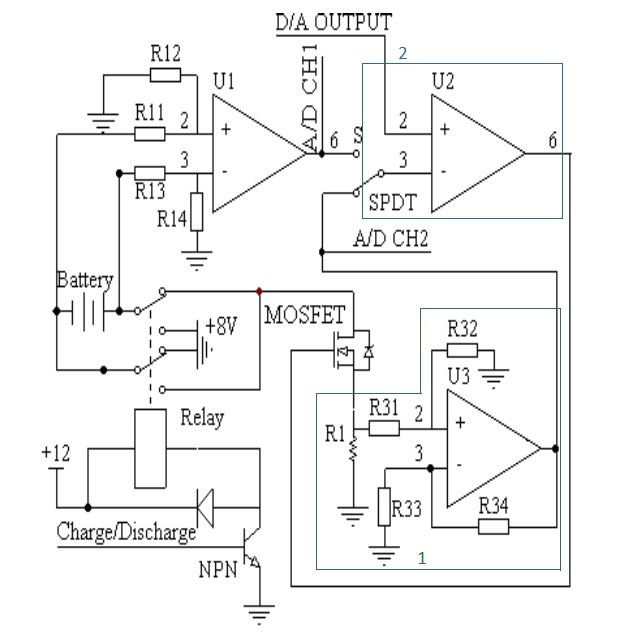
\includegraphics[width=12cm]{CAP2_diagcargaydescarga.jpg}
\caption{Diagrama de un circuito de carga y descarga de baterías~\cite{Qiu2007}.}
\label{fig:diagcargaydescarga}
\end{center}
\end{figure}

Dado que las tres topologías presentadas en las figuras~\ref{cktoreferencia} y \ref{diagcargaydescarga}   pertenecen a sistemas diferentes, es normal encontrar ciertas diferencias. Sin embargo, se rescata las similitudes entre ellos, las cuales fueron resaltadas en cuadro verdes y azules. Todas las topologías presentaron un transistor, sea NPN o Mosfet canal N, que lo utilizan para establecer la corriente constante debido a las características que éstos presentan. Así mismo, el cuadro verde representa la etapa de activación del transistor cuyo componente electrónico es el OpAmp y el cuadro azul representa la realimentación del sistema cuya función es fijar un voltaje en la carga de tal manera que pase una corriente constante en todo el tiempo de la descarga \cite{Ping2012}, \cite{Qiu2007} . \\

Por lo tanto, el circuito de control de descarga a corriente constante se podría simplificar de la siguiente manera: 

\begin{figure}[!ht]
\begin{center}
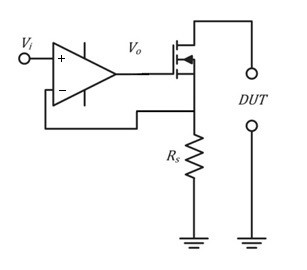
\includegraphics[width=12cm]{CAP2_cktodescarga.jpg}
\caption{Circuito de control de descarga a corriente constante. Elaborado por el autor.}
\label{fig:cktodescarga}
\end{center}
\end{figure}

El funcionamiento consiste en tener un OpAmp trabajando de forma lineal de tal manera que al fijar un voltaje en la entrada no inversora ( ) se pueda obtener el mismo valor de voltaje en la entrada inversora. Esto permitiría tener un voltaje estable en la carga  , el cual obligaría consumir una corriente constante de la batería (Device Under Test, DUT). Sin embargo, esto solo sucede cuando el transistor está activado y se encuentre en la región activa o región de saturación, ya sea un transistor BJT o un Mosfet respectivamente.

\section{Evaluación de la incertidumbre}

Usualmente se utilizan los componentes electrónicos con sus valores nominales para el diseño de un circuito electrónico; sin embargo, existe una tolerancia asociada a todos los componentes ya que ninguno es ideal, el cual produce una incertidumbre de medida en el circuito. Por lo tanto, se debe profundizar en los conceptos de incertidumbre típica ya que nuestro diseño involucra aspectos de medición.

Primero se identifican las fuentes y tipos de error que existen en las medidas. Éstas pueden ser efectos aleatorios o efectos sistemáticos. Además, esporádicamente pueden aparecer lecturas absurdas, también conocido como lecturas aberrantes. Las lecturas aberrantes son aquellas que rara vez aparecen en la muestra de datos y representan un valor totalmente equivocado de la muestra en general. Por ello, lo recomendable es separar estas lecturas de la muestra de datos adquiridos \cite{Angel2006}.

Una vez descartadas las lecturas aberrantes, una lectura $q_i$ de una magnitud $q$  se puede modelar de forma general como se muestra en la ecuación \ref{eq:lecturamagnitud}.

\begin{equation}
q_i = q + b(q) + \chi(q,i)
\label{eq:lecturamagnitud}
\end{equation}

Donde $b(q)$  es el efecto sistemático y $\chi(q,i)$  es el efecto aleatorio. Por un lado, el efecto sistemático está constituido por aquellos errores generados por derivas en el instrumento debido a factores que no se pueden controlar (envejecimiento, temperatura, entre otros) o son inherentes al método de medida (efecto de carga). En caso de que se conozca su presencia se debe intentar corregirse antes de analizar la incertidumbre en la medida. Por otro lado, los efectos aleatorios se caracterizan a partir de su función de distribución de probabilidad, tienen valores acotados y su esperanza matemática es nula. Una vez se hayan rechazado las lecturas aberrante y corregido los efectos sistemáticos, la única diferencia entre las lecturas y la magnitud que desea medirse se debe a los efectos aleatorios. El promedio de varias lecturas reduce los efectos aleatorios si es que las lecturas son estadísticamente independientes~\cite{Angel2006}. En la figura~\ref{fig:tiposdeerror} se puede apreciar algunos ejemplos para los diferentes tipos de error mencionados.

\begin{figure}[!ht]
\begin{center}
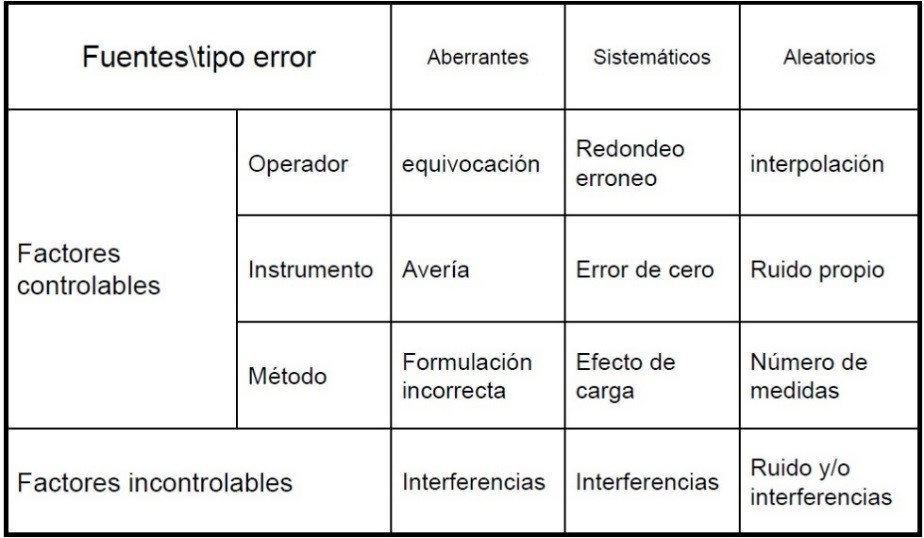
\includegraphics[width=12cm]{CAP2_tiposdeerror.jpg}
\caption{Ejemplos de tipo de error para lecturas aberrantes, efectos sitemáticos y efectos aleatorios~\cite{Angel2006}}
\label{fig:tiposdeerror}
\end{center}
\end{figure}

Según la guía para la expresión de la incertidumbre de medida, realizada por el Centro Español de Metrología (CEM) ~\cite{CENTROESPANOLDEMETROLOGIA2008}, existen dos métodos de evaluación de la incertidumbre típica.

	\subsection{Evaluación tipo A de la incertidumbre típica}

	Esta evaluación se basa en métodos estadísticos y requiere de un conjunto de medidas. Para que el método sea válido, las condiciones de las medidas no deben cambiar a lo largo de la prueba. Además, las diferentes lecturas deben ser estadísticamente independientes entre sí~\cite{CENTROESPANOLDEMETROLOGIA2008}. Por lo tanto, los pasos que se deben 			realizar para determinar la incertidumbre típica mediante este método son los siguientes:

	\begin{enumerate}
	\item Corregir los efectos sistemáticos
	\item Tomar N medidas independientes
	\item Eliminar las lecturas aberrantes
	\item Calcular la media aritmética 		% Falta poner ecuacion
	\item Calcular la desviación típica ajustada	% Falta poner ecuacion
	\item Determinar la incertidumbre típica		% Falta poner ecuacion
	\end{enumerate}

	Este método es especialmente útil con el prototipo del instrumento ya que se van adquirir muchas cantidades de muestras por un periodo de tiempo. A partir de este método se determinará la incertidumbre típica o desviación típica experimental de la medida para luego ser comparado con la incertidumbre que se determinó en el diseño del instrumento. 

	\subsection{Evaluación tipo B de la incertidumbre típica}

	La evaluación tipo B de la incertidumbre típica está más orientado a estimar magnitudes que no son obtenidas a partir de un conjunto de medidas. Es decir que, a través de métodos de estadística, se estima la incertidumbre de una magnitud a partir de toda la información disponible que se tenga de ésta. Para el diseño de un circuito, que realiza la estimación de la capacidad eléctrica de una batería, es posible utilizar este método de evaluación ya que la magnitud a estimar está relacionada por conceptos matemáticos-eléctricos~\cite{CENTROESPANOLDEMETROLOGIA2008}. \\

	Los pasos a realizar para determinar la incertidumbre típica de la capacidad eléctrica que puede proveer una batería son los siguientes~\cite{CENTROESPANOLDEMETROLOGIA2008}:	

	\begin{enumerate}
	\item Identificar todas las variables independientes eléctricas entre sí que estén relacionadas con la magnitud a estimar
	\item Asignar una función de probabilidad a cada variable eléctrica identificada y hallar su incertidumbre típica
	\item Hallar el coeficiente de sensibilidad decada variable eléctrica identificada
	\item Luego se debe obtener la incertidumbre de cada variable independiente multiplicando su incertidumbre típica con su respectivo coeficiente de sensibilidad
	\item Determinar la incertidumbre típica de la magnitud a estimar por medio de la raíz cuadrada de la suma de cada incertidumbre independiente al cuadrado.
	\end{enumerate}


\section{Estándares para descarga de baterías}

Los instrumentos de medición y descargas de baterías son regidos por estándares a nivel internacional que son establecidos por organizaciones como IEC (International Electrotechnical Commision), ANSI (American National Standards Institute), SAE (Society of Automotive Engineers), entre otros. 

El prototipo que se diseñará en la presente tesis no tendrá como objetivo obtener certificados oficiales por parte de estas organizaciones. Sin embargo, se toma en consideración que existen estos estándares con la finalidad de obtener los mejores resultados posibles. En la tabla 5 se muestra los diferentes estándares que se aplicaría al instrumento de medición. 

%Falta poner la tabla







